\documentclass[journal]{IEEEtran}
\usepackage{amsmath,amssymb,amsfonts}
\usepackage{graphicx}
\usepackage{cite}
\usepackage{booktabs}
\usepackage{caption}
\usepackage{array}
\usepackage{float}
\usepackage{pdflscape}
\usepackage{longtable}
\usepackage{geometry}
\usepackage{pdflscape}
\usepackage{longtable}
\usepackage{fancyhdr}
\usepackage{float}
\usepackage{graphicx}
\usepackage{amsmath}
\usepackage{amsfonts}
\usepackage{lineno}
\usepackage{array}
\usepackage{booktabs}
\usepackage{caption}

% pandoc writeup.md --template=mytemplate.tex -o output.pdf --bibliography=refs.bib --pdf-engine=pdflatex --citeproc --csl=ieee.csl



\title{Lite Learning: Efficient Crop Classification in Tanzania Using Feature Extraction with Machine Learning \& Crowd Sourcing}

\author{
    Michael L. Mann, 
    Lisa Colson,
    Rory Nealon,
    Ryan Engstrom,
    Stellamaris Nakacwa
    \thanks{Michael L. Mann and Ryan Engstrom are with The George Washington University, Washington DC 20052 (e-mail: mmann1123@gmail.com).}
    \thanks{Lisa Colson is with the USDA Foreign Agricultural Service, Washington DC 20250.}
    \thanks{Rory Nealon is with USAID GeoCenter, Washington DC 20523.}
    \thanks{Stellamaris Nakacwa is with YouthMappers, Texas Tech University, Lubbock TX 79409.}
}

\begin{document}

\maketitle

\begin{abstract}
This study introduces a novel approach to traditional machine learning methodology for crop type classification in Tanzania, by integrating crowdsourced data with time-series features extracted from Sentinel-2 satellite imagery. Leveraging the YouthMappers network, we collected ground validation data on various crops, including challenging types such as cassava, millet, sunflower, sorghum, and cotton across a range of agricultural areas. Traditional machine learning algorithms, augmented with carefully engineered time-series features, were employed to map the different crop classes. Our approach achieved high classification accuracy, evidenced by a Cohen's Kappa score of 0.82 and an F1-micro score of 0.85. The model often match or outperform broadly used land cover models which simply classify 'agriculture' without specifying crop types. By interpreting feature importance using SHAP values, we identified key time-series features driving the model's performance, enhancing both interpretability and reliability. Our findings demonstrate that traditional machine learning techniques, combined with computationally efficient feature extraction methods, offer a practical and effective “lite learning” approach for mapping crop types in data-scarce environments. This methodology facilitates accurate crop type classification using a low-cost, resource-limited approach that contributes valuable insights for sustainable agricultural practices and informed policy-making, ultimately impacting food security and land management in resource-limited contexts, such as sub-Saharan Africa.
\end{abstract}

\begin{IEEEkeywords}
Remote sensing, machine learning, crop classification, time-series analysis, crowdsourcing, Sentinel-2, feature engineering.
\end{IEEEkeywords}

\section{Introduction}
\subsection{Background and Context}

The free access to remotely sensed data, such as imagery from satellites (e.g. Sentinel-2, Landsat), has allowed for crop type classification in developing countries. By leveraging the power of advanced imaging technologies combined with machine learning algorithms, researchers and practitioners can now identify and map different crop types over large geographic areas at no or low cost \cite{hersh2021open}. This has the potential to improve food security, land use planning, and agricultural policy in regions where ground-based data collection is limited or non-existent \cite{rs10010099, li2023development, ibrahim2021mapping}.

In recent years, machine learning approaches have emerged as powerful tools for crop type classification using remotely sensed data. Specifically, methods based on machine learning algorithms have gained recognition for their effectiveness in matching valuable spectral information from satellite imagery to observations of crop type for particular locations. Machine learning algorithms, including decision trees, random forests, support vector machines (SVM), and k-nearest neighbors (KNN), have been successfully used to  classify imagery into unique agricultural types \cite{ibrahim2021mapping, begue2018remote, delince2017handbook}. These algorithms leverage the rich spectral information captured by satellite sensors, allowing them to identify distinctive patterns associated with different crop types. By training on large labeled datasets where ground-validation information on crop types is linked to corresponding image pixels, these models can effectively learn the relationships between the spectral characteristics of crops and their respective classes \cite{rs10010099}.

The strength of traditional machine learning approaches lies in their ability to exploit both the spectral and time-series patterns within the remotely sensed data. Traditional machine learning approaches offer advantages in terms of interpretability and computational efficiency compared to deep learning architectures. They provide insight into the decision-making process and can be more readily understood and explained by domain experts. Additionally, these methods are generally less computationally demanding and require less training data, making them suitable for applications with limited computational resources \cite{hohl2024recent, rs13132591, agriculture13050965, LI2023103345, MA2019166}.
 

Traditional machine learning algorithms require the extraction of variables (e.g. max EVI, mean blue band) that can help distinguish different plant or crop types \cite{begue2018remote}. The development of salient time-series features to capture phenological differences between locations from remotely sensed images remains a challenge. These features are typically derived from the spectral bands (e.g. red edge, NIR) of the satellite imagery or indexes, such as the enhanced vegetation index (EVI), and basic time series statistics (e.g. mean, max, minimum, slope) for the growing season \cite{morton2006cropland}. Meanwhile a broader set of time series statistics from bands or indexes may be more relevant for a number of applications. For instance the skewness of EVI might help distinguish crops that green-up earlier vs later in the season, measures of the numbers of peaks in EVI might help differentiate intercropping or multiple plantings in a season \cite{begue2018remote}. However, the selection and extraction of these features can be time-consuming and labor-intensive, requiring domain expertise and manual intervention.

In contrast, deep learning methods have dominated the most recent literature \cite{agriculture13050965, hohl2024recent}. These methods include both recurrent neural networks (RNN) and convolutional neural networks (CNN). Recurrent Neural Networks (RNNs) are a class of neural networks that are particularly powerful for modeling sequential data such as time series, speech, text, and audio. The fundamental feature of RNNs is their ability to maintain a 'memory' of previous inputs by using their internal state (hidden layers), which allows them to exhibit dynamic temporal behavior. RNNs and its variants allow the integration of time-series imagery, significantly improving crop type classification outcomes especially in data rich environments \cite{agriculture13050965, camps2021deep}. Deep learning approaches however typically require much larger sets of training data, may be more prone to overfitting especially with small sample sizes, have significant limitations to interpretability, and require expensive compute \cite{hohl2024recent, rs13132591, agriculture13050965, LI2023103345, MA2019166}. Although recent efforts have closed the gap e.g. \cite{tseng2021cropharvest}, the lack of readily available and reliable ground truth data or benchmark datasets for training, as discussed earlier, may limit the applicability of deep learning for a variety of tasks including crop classification and make researchers more reliant of less reliable techniques like transfer learning or zero-shot or low shot methods \cite{owusu2024towards, LI2023103345, MA2019166}. Moreover, training data for extreme events, like crop losses, disease, and lodging are largely non-existant.  Interpretability is also a salient weakness as interpretation of models allows us to gain scientific insight and assess trustworthiness and fairness in so far as outputs affect policy decisions.  

An alternative approach turns back the clock on deep learning approaches. For instance CNN classifiers, through the exertion of tremendous effort of GPUs, can apply and learn from thousands of filters or convolutions that help detect distinct features like edges, textures or patterns. It is however possible to apply a more limited yet salient set of filters like Fourier Transforms, Differential Morphological Profiles \cite{pesaresi2001new}, Line Support Regions or Structural Feature Sets \cite{huang2007classification} amongst others, to images and then use these as features in more traditional machine learning approaches \cite{graesser2012image, owusu2024towards, engstrom2022poverty, chao2021evaluating, urbansci7040116}. This approach may be particularly useful in data-scarce environments, requiring less training data and potentially offering more efficient results in low-information settings. The same approach has been taken for time series analysis, where instead of learning patterns through a RNNs memory, we can apply a more limited but potentially salient series of time series filters. Measures of trends, descriptions of distributions, or measures of change and complexity might adequately describe time series properties for regression and classification tasks \cite{christ2018time, yang2021anomaly}. This time series filter approach, developed for this paper, can also be applied on a pixel-by-pixel basis to satellite image bands or index values \cite{xr_fresh_2021}.

Field-collected data provides the necessary validation and calibration for remote sensing-based models. It serves as the benchmark against which the model's predictions are evaluated and refined. Ground validation data collected through field visits, observation, and interactions with local farmers offers essential insights into the specific crop types present in the study area. Validating and training models with accurate ground reference information allows for the spectral patterns captured by remote sensing data to be correctly associated with the corresponding crop. By combining the spectral information from satellite imagery with ground validation data, researchers can develop robust models that effectively differentiate between different crop types based on their unique spectral signatures and temporal patterns.

The collection of field observations and ground validation data is a critical input for the development of models to classify crop types \cite{delince2017handbook, MA2019166}. However, obtaining accurate and timely ground validation data can be challenging in developing countries due to limited resources, infrastructure, and local capacity \cite{delince2017handbook, begue2018remote}. In many cases, researchers rely on crowdsourced data from volunteers or citizen scientists to supplement or validate ground truth data collected through traditional methods. Projects like \cite{tseng2021cropharvest} point to the paucity of multi-class crop type datasets globally. This is a significant gap in the field of crop type classification, as the availability of high-quality training data is essential for the development of accurate and reliable machine learning models \cite{rs13132591}.
 

In this study we aim to address two critical challenges in the field of crop type classification: the lack of in-season multi-class crop type datasets, and the need for new methods to obtain high accuracy crop type predictions from limited amounts of training data.
 
We propose a novel approach that combines crowdsourced data with a new automated approach to extracting time-series features from satellite imagery. We apply this new approach to classify crop types in Northern Tanzania. By leveraging the power of crowdsourcing and remote sensing technologies, we aim to develop a robust and scalable solution for crop type classification that can be adapted to other regions and contexts with a minimal or no cost.
 

\section{Data \& Methods}
Data for this study were collected from multiple sources, including satellite imagery, and crowdsourced ground truth observations. The section below describes the input data and methods used throughout the paper.

\subsection{Study Area}
The study was conducted in 50 wards within three major districts of Arusha, Dodoma and Mwanza in Tanzania as seen in Figure \ref{fig:study_area}. Tanzania, a country in East Africa, is known for its diverse agricultural landscape.  The region is characterized by a mix of smallholder farms, commercial plantations, and natural vegetation, making it an ideal yet challenging location for studying crop type classification. Our choice of these three districts was driven by the distinct variation in the major crop types that possibly dominated in each district,among oil seeds, grains and commercial crops such as cotton.

\begin{figure}[!t]
   \centering   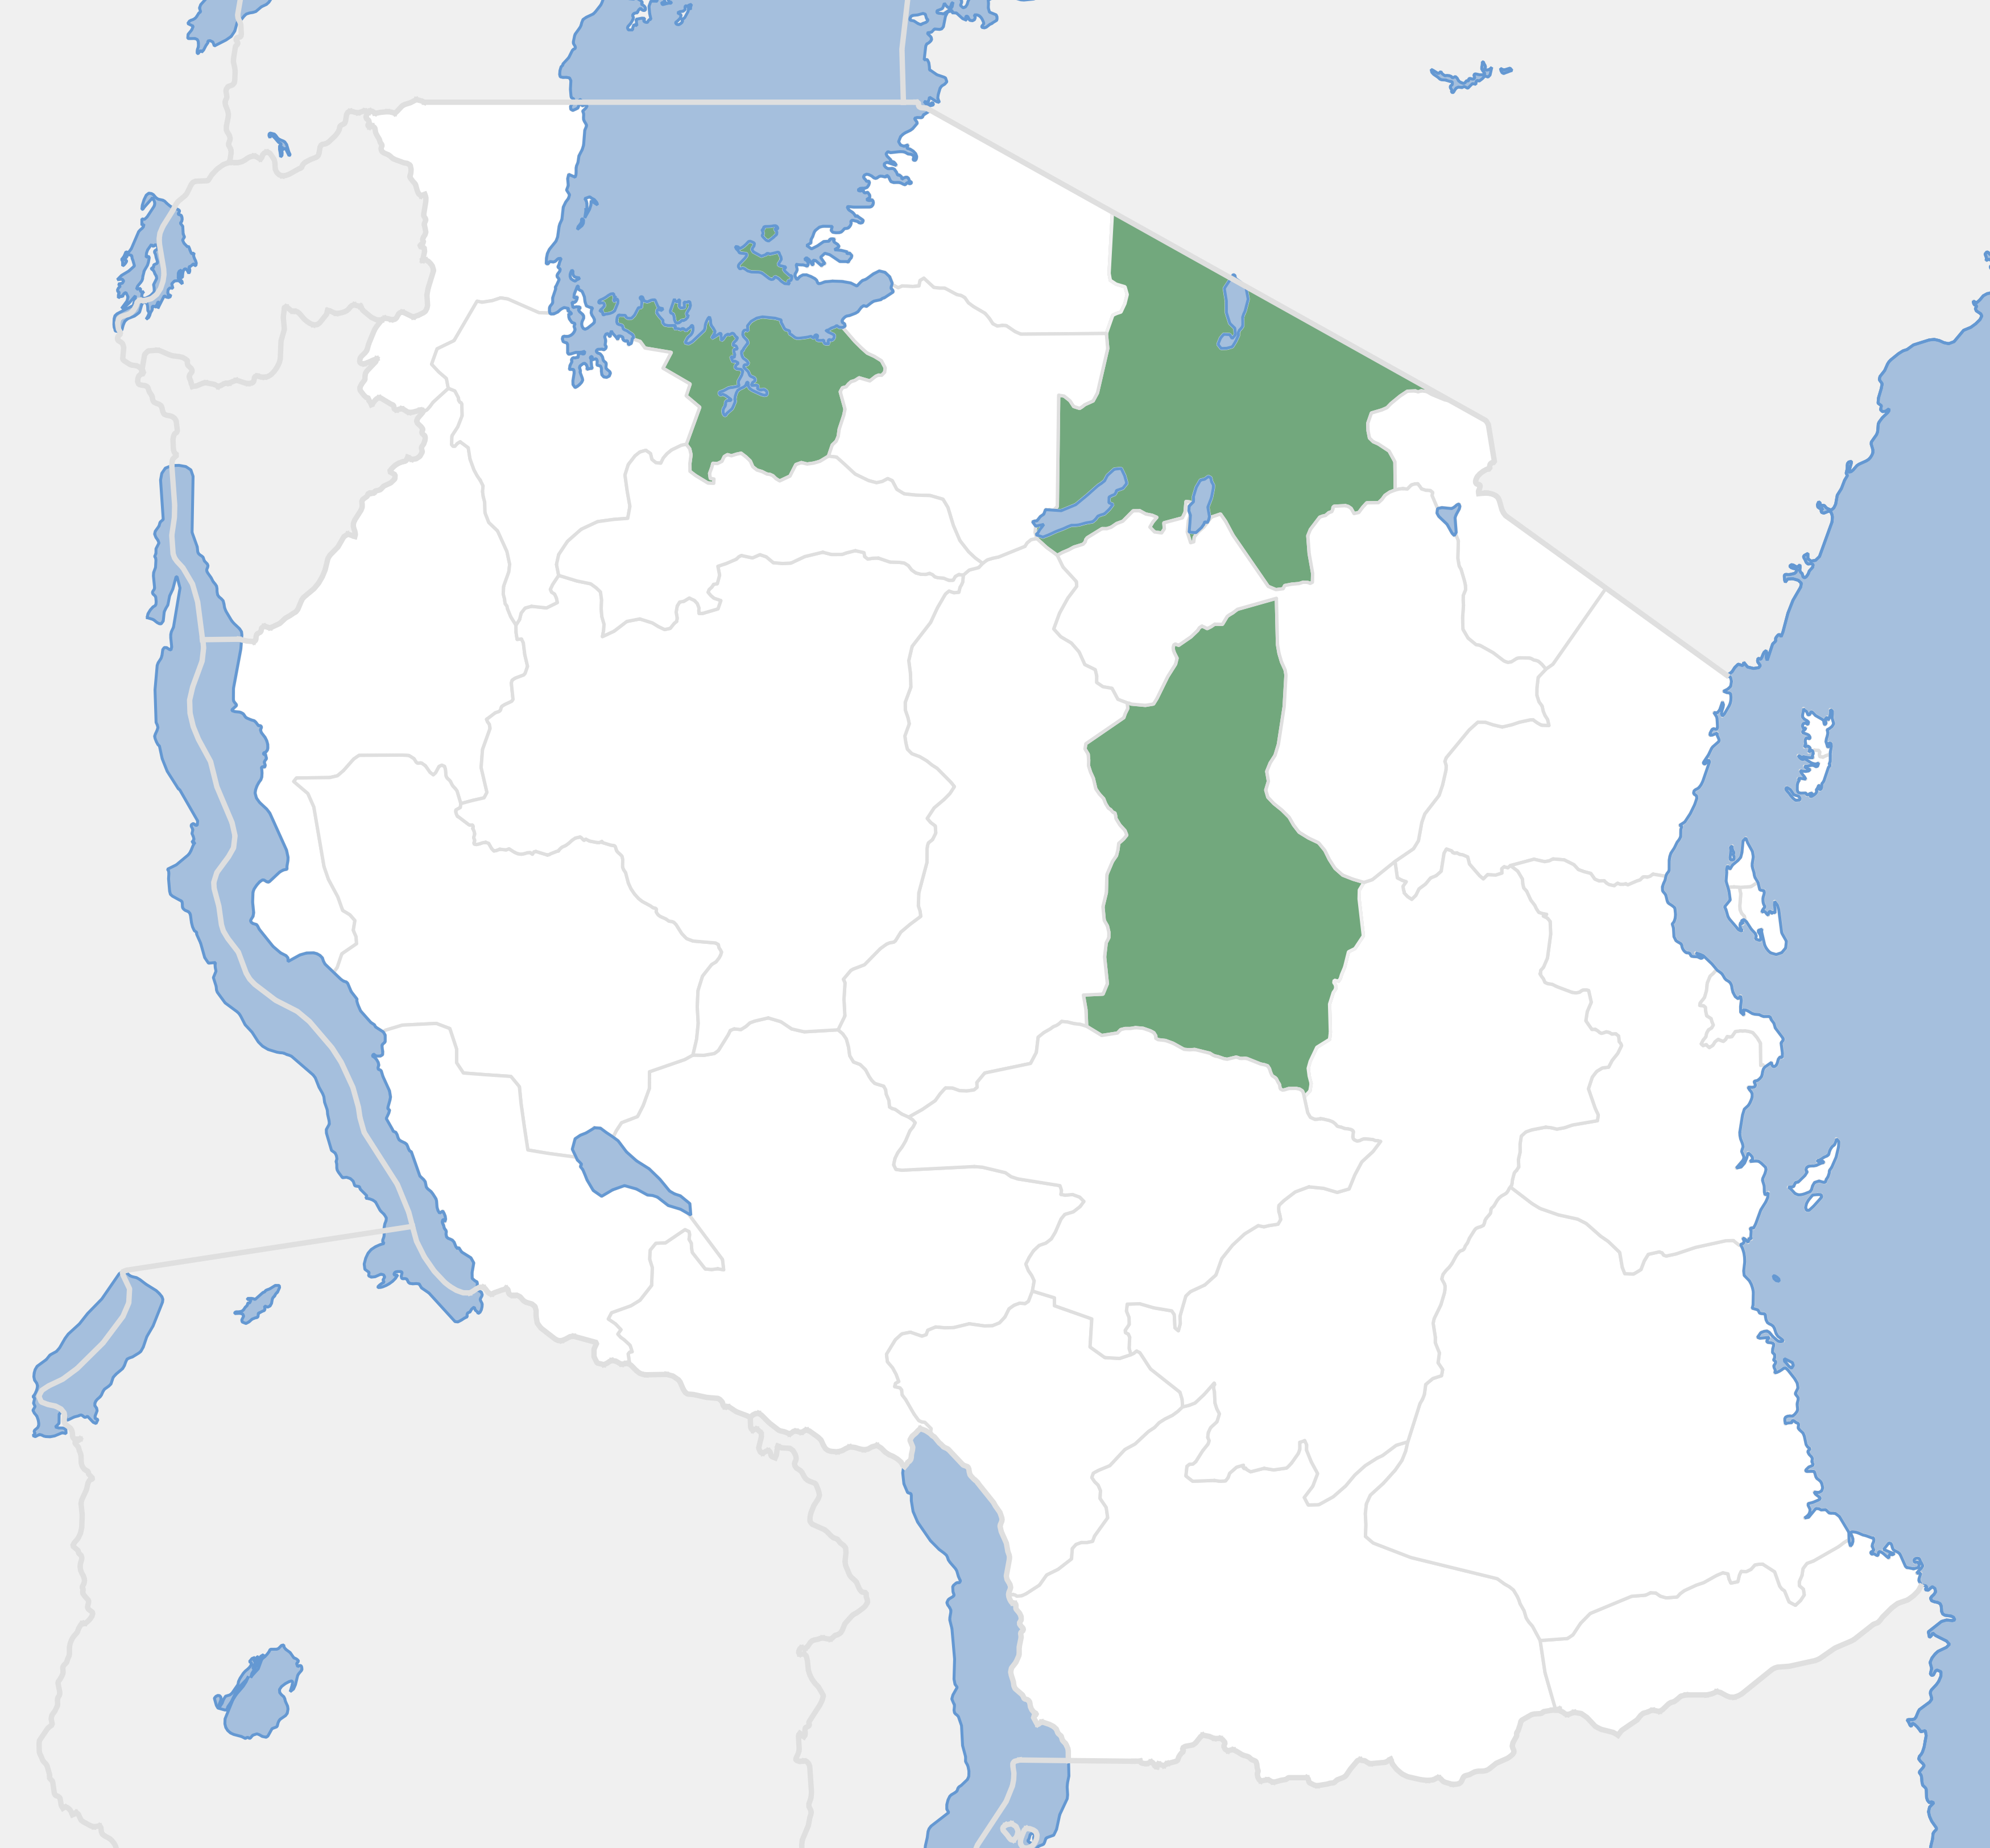
\includegraphics[width=0.8\linewidth]{/home/mmann1123/Documents/github/YM_TZ_crop_classifier/writeup/figures/tz_ym_crop_target_provinces.png} 
   \caption{Study area map \newline Districts in Northern Tanzania where field visits were carried out (green)}
   \label{fig:study_area} %can refer to in text with \ref{fig:study_area}
\end{figure}

\subsection{Crowd Sourced Data Collection}
Crop type data collection was designed and executed by YouthMappers through a crowdsourced GIS approach. The method was designed in 3 steps where: 1) Development of and training all intended student participants. 2) Data collection using KoboToolbox hosting a well developed data model. The exercise lasted 14 days with 7 days of iterative pilot testing on different farms, crops and landscapes. Finally the last step, 3) was the data review and cleaning phase to generate a sample for training.

Additional training data was collected utilizing high resolution imagery from Google Earth. These data were used to supplement the crowdsourced data and improve the model's ability to distinguish between crops and more common land cover types like forests, urban areas, and water.  The final cleaned dataset includes 1,400 crop type observations of rice, maize, cassava, sunflower, sorghum, cotton, and millet; plus 386 other observations of land cover classes including water, tidal areas, forest, shrub and urban.  

\subsubsection{Data Collection Methods}

To ensure the success of our project, we focused heavily on the design of our data collection methods. These methods were carefully integrated, taking into account: the crop calendar, information on the different stages of crop development, the distances between crop fields, the tools used, and data quality assurance.

Young crops exhibit significant differences compared to mature crops in terms of color, density, and phenological development. Variations in the crop cycle across different fields could lead to heteroscedasticity in the spectral reflectance measurements used for machine learning (ML) training, thereby affecting the precision and accuracy of the model. By targeting the period of April through May we aimed to capture crops late in the growing season and yet before harvest as seen in the crop calendar in Figure \ref{fig:crop_cal} below.

\begin{figure}[!t] 
   \centering   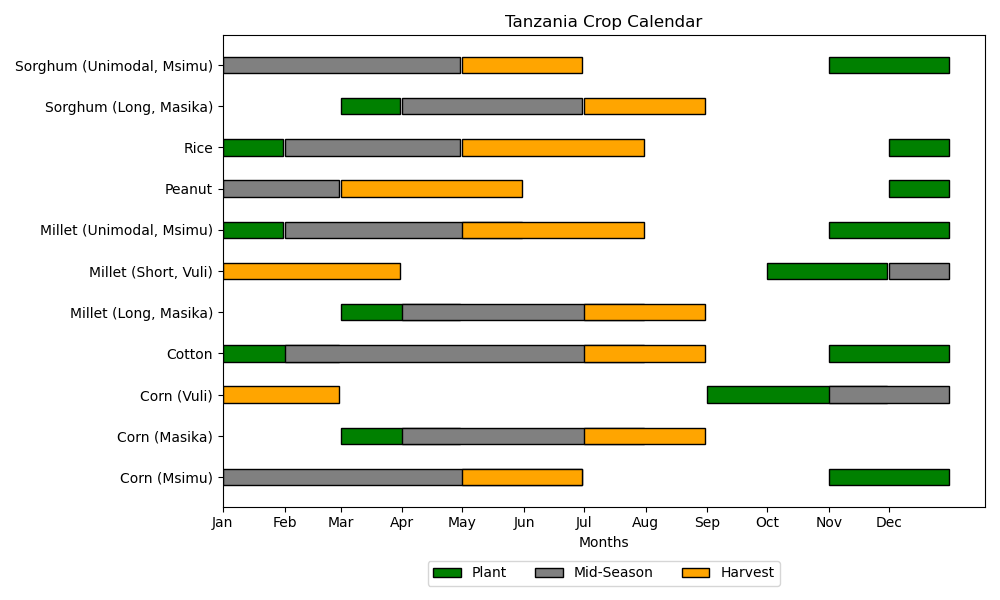
\includegraphics[width=0.8\linewidth]{/home/mmann1123/Documents/github/YM_TZ_crop_classifier/writeup/figures/plant_ghant.png}
   \caption{Tanzania Crop Calendar }
   \label{fig:crop_cal} %can refer to in text with \ref{fig:crop_cal}
\end{figure} Source: \cite{cc_tanzania}

USDA’s Foreign Agricultural Service compiles information on planting and harvest windows for grain, oilseed, and cotton crops as an important tool to support crop condition assessments with satellite imagery. Tanzania’s crop planting seasons are shaped by its bimodal and unimodal rainfall patterns, which vary by region. In the north and northeast, bimodal areas experience the short rains (Vuli) from late-October to mid-January, during which crops like maize, beans, and vegetables are planted in October and November, and the long rains (Masika) from March to May, supporting crops like maize, rice, sorghum, and cassava, typically planted in February and March. In the central, southern, and western regions with unimodal rainfall, there is a single rainy season from November to April, when crops such as cotton, maize, millet, rice, and sunflower are planted in November and December. This diversity in rainfall patterns allows for a wide variety of crops suited to the local climate and seasonal conditions.

The data collection took place between late April and May as shown in figure \ref{fig:crop_cal} to align with mid-season for many crops. YouthMappers were advised to focus on a set of target crops, ones known to be present in the region and at appropriate crop growth stages. Before embarking on data collection, discussions covered several factors to consider in selecting field collection sites. Factors included field size to establish a minimum detectable by the satellite imagery, clear and open fields to enhance clean spectra sampling, prioritizing areas covered by a single crop to reduce confusion, sampling distribution of at least one kilometer between stops, and even crop maturity and health. YouthMappers were advised to identify only fields 30 meters or greater across to ensure a minimum size detectable by the satellite imagery. When picking between fields for data collection, defining clear and open fields was discussed with several examples, as agriculture can include mixed land cover types with tree cover, power lines, buildings, and other obstructions that prevent the satellite from cleanly capturing spectra of only the crop. YouthMappers were advised to only pick clear and open fields and prioritize those growing only one crop. The recommendation to have a sampling distribution of at least one kilometer was a compromise between the amount of time available for data collection, the expense of travel, and a sufficient distribution to reduce spatial autocorrelation. It was permitted for YouthMappers to identify adjacent fields growing different types of crops, but otherwise highly encouraged for them to return to the vehicle and drive the 1 km to collect more data. The most important factors driving the timing for data collection were crop maturity and health. The fieldwork was conducted between late-April to May 2023 because the target crops typically reach reproductive stages with maximum canopy cover during this time of year. This crop stage is best suited for discerning different crop types with satellite imagery. While most fields were found in late reproductive stages, drought conditions impacted the health of some fields. YouthMappers were advised to prioritize and identify mature, lush green fields, as ideal data collection sites. By thoroughly discussing each of these factors, we trained YouthMappers to select fields best suited as in-situ training data for satellite imagery analysis.

The data collection was managed through KoboCollect, hosted on the KoboToolBox infrastructure, which provided an effective platform for gathering and organizing data. This approach enabled a collection of the desired volume of data points necessary for model training and evaluation, as summarized in Table \ref{tab:data_n}.
 
\begin{table} 
\centering
\begin{tabular}{@{}lp{1cm}p{2cm}p{2cm}@{}}
\toprule
& \textbf{Arusha} & \textbf{Mwanza} & \textbf{Dodoma} \\ \midrule
\textbf{Desired points:} & \textbf{300} & \textbf{1000} & \textbf{800} \\ 
\midrule \\
\textbf{Crops:} & Maize \newline Rice \newline Sorghum \& Millet 
               & Maize \newline Cotton \newline Rice \newline Peanuts/Groundnut 
               & Sorghum \newline Maize \newline Millet \newline Sunflower \newline Peanuts/Groundnut \newline Cotton Fields \\ 
\bottomrule
\end{tabular}
\caption{Collection Targets and Primary Crops by Region in Tanzania}
\label{tab:data_n}
\end{table} 

\subsection{Satellite Imagery}

Satellite imagery was obtained from the Sentinel-2 satellite constellation, which provides high-resolution multispectral data at 10-meter spatial resolution. The imagery was acquired over the study area  between January and August of 2023 during the growing season, capturing the spectral characteristics of different crop types and coinciding with field data collection. The Sentinel-2 L2 harmonized reflectance data were pre-processed to remove noise and atmospheric effects, ensuring that the spectral information was accurate and reliable for classification purposes \cite{begue2018remote}.

In our study, cloud and cloud shadow contamination was mitigated using the \texttt{s2cloudless} machine learning model on the Google Earth Engine platform. Cloudy pixels were identified using a cloud probability mask, with pixels having a probability above 50\% classified as clouds. To detect cloud shadows, we used the Near-Infrared (NIR) spectrum to flag dark pixels not identified as water as potential shadow pixels. The projected shadows from the clouds were identified using a directional distance transform based on the solar azimuth angle from the image metadata. A combined cloud and shadow mask was refined through morphological dilation, creating a buffer zone to ensure comprehensive coverage. This mask was applied to the Sentinel-2 surface reflectance data to exclude all pixels identified as clouds or shadows, enhancing the reliability of the dataset for environmental analysis.

Monthly composites were collected for January through August of 2023 for the the bands B2 Blue (458-523nm), B6 Vegetation Red Edge (733-738nm), B8 Near Infrared (785-899nm), B11 Short-Wave Infrared (SWIR)(1565-1655nm), and B12 Short Wave Infrared (2100-2280nm). Sw. We also calculate the Enhanced Vegetation Index (EVI) and hue, the color spectrum value \cite{GoogleHSV}. This computed hue value provides the basic color as perceived in the color wheel, from red, through green, blue, and back to red for each pixel. Due to the high prevalence of clouds in the region, linear interpolation was used to fill in missing data in the time series using \texttt{xr\_fresh} \cite{xr_fresh_2021}. These bands were selected based on their relevance to crop type classification and their ability to capture the unique spectral signatures of different crops. The monthly composites were used to generate time series features for each pixel in the study area, providing valuable information on the temporal dynamics of crop growth and development.

\subsection{Time Series Features}

Time series features capture the temporal dynamics of crop growth and development, providing valuable information on the phenological patterns of different crops. We leverage the time series nature of the satellite imagery to extract relevant features for crop type classification.

In this study, we utilized the \texttt{xr\_fresh} toolkit to compute detailed time-series statistics for various spectral bands, facilitating comprehensive pixel-by-pixel temporal analysis (Mann, Michael L. 2024). The \texttt{xr\_fresh} framework is specifically designed to extract a wide array of statistical measures from time-series data, which are essential for understanding temporal dynamics in remote sensing datasets.

The metrics computed by \texttt{xr\_fresh} in this study include basic statistical descriptors, changes over time, and distribution-based metrics, applied to each pixel's time series for selected spectral bands (B12, B11, hue, B6, EVI, and B2). The list of computed time-series statistics encompasses:

\begin{itemize}
\item
  \textbf{Energy Measures}: Absolute energy which provides a sum of squares of the values.
\item
  \textbf{Change Metrics}: Absolute sum of changes to quantify overall variability, mean absolute change, and mean change.
\item
  \textbf{Autocorrelation}: Calculated for three lags (1, 2, and 3) to assess the serial dependence at different time intervals.
\item
  \textbf{Count Metrics}: Count above and below mean, capturing the frequency of high and low values relative to the average.
\item
  \textbf{Extreme Values}: Day of the year for maximum and minimum values, providing insight into seasonal patterns.
\item
  \textbf{Distribution Characteristics}: Kurtosis, skewness, and quantiles (5th and 95th percentiles) to describe the shape and spread of the distribution.
\item
  \textbf{Variability Metrics}: Standard deviation, variance, and whether variance is larger than standard deviation to evaluate the dispersion of values.
\item
  \textbf{Complexity and Trend Analysis}: Time series complexity and symmetry looking, adding depth to the analysis of temporal patterns.
\end{itemize}

For a full list of the time series features extracted in this study and their descriptions, please refer to the Appendix.

The integration of \texttt{xr\_fresh} into our analytical workflow allowed for an automated and robust analysis of temporal patterns across the study area. By leveraging this toolkit, we could efficiently process large datasets, ensuring that each pixel's temporal dynamics were comprehensively characterized, which is critical for accurate environmental monitoring and change detection.


\subsection{Data Extraction}

To partially account for variation in field size we extracted pixels based on a buffer around field point locations. This allows us to account for the fact that fields likely represent groups of adjacent pixels. Small fields were buffered by only 5 meters, medium fields by 10m and large fields by 30m. This approach allowed us to capture the time series features from the surrounding area, providing a more comprehensive representation of the field's characteristics. The use of larger buffers was explored but found to decrease model performance as fields tended to be heterogenous - for instance containing patches of trees. To account for this in our modeling we treat observations from the same field as a "group" in our cross-validation scheme - as described below.

\subsection{Machine Learning Models}

In our study, we utilized the extracted time-series features from satellite imagery, described above, to analyze crop classifications.  Notably, features were centered and scaled from the \texttt{scikit-learn} library to normalize the data, followed by the application of a variance threshold method to reduce dimensionality by excluding features with low variance \cite{scikit-learn}.

We employ \texttt{Optuna}, an optimization framework, to conduct systematic model selection and hyperparameter tuning \cite{optuna_2019}. Our methodology involved defining a study using Optuna where each trial proposes a set of model parameters aimed at optimizing performance metrics. Specifically, we used stratified group k-fold cross-validation with the number of splits set to three, ensuring that samples from the same field were not split across training and validation sets to prevent data leakage. The scoring metric utilized is the kappa statistic, chosen for its suitability in evaluating models on imbalanced datasets.

This approach allows us to rigorously evaluate and compare different classifiers, including LightGBM, Support Vector Classification (SVC), and RandomForest, and their configurations under a variety of conditions. The final selection of the model and its parameters was based on the ability to maximize the kappa statistic, ensuring that the chosen model provided the best possible performance for the classification of land cover types in our dataset.

\subsection{Interpretation and Feature Selection}

To interpret the contributions of individual features to the model predictions, we employed SHapley Additive exPlanations (SHAP) \cite{shaps_2017}. This approach, based on game theory, quantifies the impact of each feature on the prediction outcome, providing insights into which features are most influential in determining land cover types.

In our feature selection process, we incorporate both the mean and maximum SHAP values to comprehensively assess the influence of features on model predictions. The mean of the absolute SHAP values across all samples, provides a measure of the average impact of each feature, highlighting its overall importance across the dataset. This approach emphasizes features that consistently affect the model’s output but might underrepresented the significance of features causing substantial impacts under specific conditions. To address this, we also consider the maximum absolute SHAP values. Sorting features by their maximum absolute SHAP values allows us to identify those that have significant, albeit possibly infrequent, effects on individual predictions. This method ensures that features crucial for particular scenarios are not overlooked, thus offering a more nuanced understanding of feature importance that balances general influence with critical, situation-specific impacts.

Feature selection then is the union of the top 30 time series features found with both the mean and maximum SHAP values, resulting in 33 total features. This approach ensures that the selected features are both consistently influential across the dataset and capable of exerting substantial impacts under specific conditions, providing a comprehensive set of features for model training and evaluation.

\section{Results \& Discussion}

\subsection{Crowd Sourced Data}

To address the significant gap in available crop type datasets, particularly in developing regions, this study harnessed the power of crowdsourced data to enhance the robustness and applicability of our machine learning models. Crowdsourced data collection, an innovative approach in the agricultural domain, involves gathering data from a large number of volunteers or citizen scientists, who provide valuable ground truth information. This method has proven especially useful in areas where traditional data collection methods are challenging due to logistical, financial, or infrastructural constraints.

By leveraging  the YouthMappers student organization, with over 420 chapters in 80 countries, we were able to collect a large dataset of crop type observations in Tanzania. Participating YouthMappers chapters included: the Institute of Rural Development Planning - Dodoma, Institute of Rural Development Planning - Mwanza, University of Dodoma, the Nelson Mandela African Institution of Science and Technology, and the Institute of Accountancy Arusha. Moreover this exercise provided an important opportunity for students to gain practical experience in data collection, analysis, and interpretation, contributing to their professional development and capacity building in the geospatial domain.

\subsubsection{Challenges and Lessons Learned}

There were a number of challenges involved with planning, and implementing a large-scale field operation. One of the primary challenges encountered was the variability in crop cycles across different fields and crop identification more generally. This was particularly true in Arusha, where fields were found in almost every stage of crop development and some fields were visited before the reproductive stages, as the drought delayed planting. In other regions, some crops had already been harvested. This discrepancy resulted in incomplete datasets, as certain crop types were missing or not easily accounted for. The absence of these crops in certain areas impacted our modeling efforts by reducing the representativeness of the training data. Second, although the YouthMappers teams did a commendable job, crop identification is challenging for non-agricultural experts. This task was even more challenging given the heterogeneity of local planting practices and the similarity of early stage growth between, for instance, crops like maize and sorghum. To mitigate this issue YouthMappers teams took detailed photos of each field. These images provided us the ability to verify crop types remotely before training the model. While extremely useful, the collection of more detailed single plant images could have helped us minimize removal of some observations. Third, the site selection depended on many non-crop related factors including where the training could be hosted and time constraints based on YouthMappers student’s academic calendars. This led to changes in which target crops were selected. Fourth, travel was finally approved during a drought year. This is helpful for transportation during field work, yet poses a challenge as more fields can be abandoned, harvested early, or otherwise found in a poor condition. To mitigate many of these issues, future data collection efforts should allow for more flexibility in the timing in data collection and ensure coverage that reflects local crop cycles.

\subsection{Land Cover and Crop Type}

The distribution of primary land cover types within the training dataset used for the model are represented in Figure \ref{fig:lc_percentages}. The dataset consists of a diverse range of land cover types, each contributing differently to the total number of observations. Maize is the most prevalent land cover type, accounting for the highest percentage of the observations, followed by rice and sunflower. This is indicative of the agricultural dominance in the region being studied. Less common land covers such as millet, sorghum, and urban areas represent intermediate percentages, reflecting the  heterogeneous landscape that includes both agricultural and urbanized zones.

\begin{figure}[!t]
   \centering   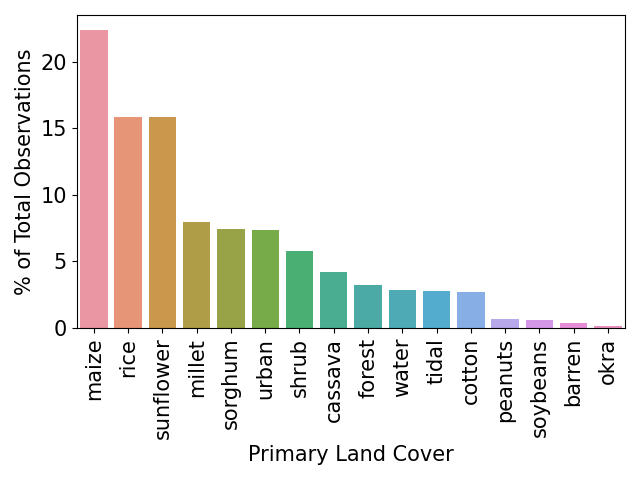
\includegraphics[width=0.8\linewidth]{/home/mmann1123/Documents/github/YM_TZ_crop_classifier/writeup/figures/primary_land_cover.png} % Adjust the path and options
   \caption{Land Cover by Percentage of Observations}
   \label{fig:lc_percentages} %can refer to in text with \ref{fig:lc_percentages}
\end{figure}

\subsection{Feature Importance}

The interpretation of model behavior using SHAP values has allowed for a deeper understanding of how different spectral features impact the model's predictions, which is critical for refining the feature selection process. By analyzing both the mean and maximum SHAP values, we were able to prioritize features based on their overall impact as well as their critical contributions to specific model decisions.

In the two summary plots below, we display the SHAP values for each feature, to identify how much impact each feature has on the model output for pixels in the validation dataset. Features are sorted by the sum of the SHAP value across all samples. The figures bar length represents the mean contributions to explaining each predicted land class value - with different land classes represented with different colors (hues). This visualization provides a comprehensive overview of the feature importance, highlighting the key predictors that drive the model's predictions. For example, features that are highly influential for "maize" may not be as impactful for "rice" or "sorghum", reflecting the unique spectral signatures of these crops.

\subsubsection{Mean SHAP Values}


In Figure \ref{fig:mean_shaps}, the mean SHAP values provide insights into the average impact of each feature across all predictions. This analysis highlights the features that consistently influence the model's output across various scenarios. For example, the mean value of B11 (B11.mean) and the 5th percentile of hue (hue.quantile.q.0.05) features were found to have substantial average impacts on model outputs, suggesting their strong relevance in distinguishing between different crop types. Reflecting on the colors of the bars we can see that 'B11.mean' is important in distinguishing sunflower, sorghum, and millet to a roughly equal degree, and has some small impact on distinguishing other classes. While 'hue.quantile.q.0.05' has the strongest effect distinguishing rice, sunflower, and to a lesser degree cotton. Looking down the list we can see that features like "EVI.standard.deviation" are most effective at isolating urban areas, and 'B12.mean.second.derivative.central' substantively differentiates shrub from other classes. Note that the mean second derivative of B12 is a measure of the rate of change of the rate of change of the B12 band over time, so positive values indicate increasing rate of change (increasingly upward trend), and negative values with decreasing rate of change (increasingly downward trend).

\begin{figure}[!t]
    \centering
    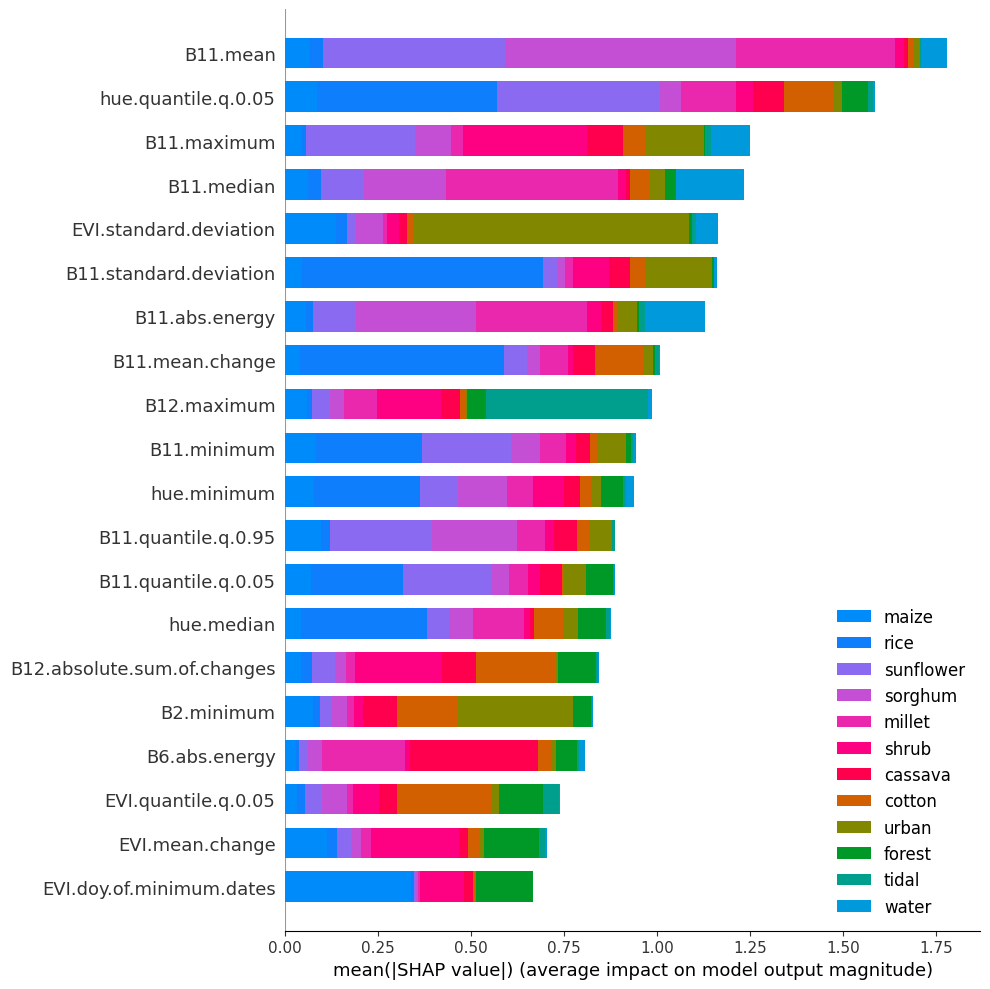
\includegraphics[width=0.8\linewidth]{/home/mmann1123/Documents/github/YM_TZ_crop_classifier/writeup/figures/mean_shaps_importance_no_other_30_LGBM_kappa_3.png} % Adjust the path and options
    \caption{Top 20 Mean SHAP Feature Importance by Land Cover Type}
    \label{fig:mean_shaps} %can refer to in text with \ref{fig:mean_shaps}
\end{figure}

\subsubsection{Max SHAP Values}
On the other hand, Figure \ref{fig:max_shaps}, maximum SHAP values uncover features that, while perhaps not consistently influential, have high impacts under particular conditions. This aspect of the analysis is crucial for identifying features that can cause significant shifts in model output, potentially corresponding to specific agricultural or environmental contexts. Features such as "hue.median" and "B11.quantial.q.0.95" show high maximum SHAP values, indicating their pivotal roles in determining certain classes. For instance,  "B11.maximum" reflects peak reflectance in the Short-Wavelength Infrared (SWIR), which could be critical in identifying crops at their maximum biomass, like sunflower at full bloom compared to other crops at different stages of growth. 

\begin{figure}[!t]
    \centering
    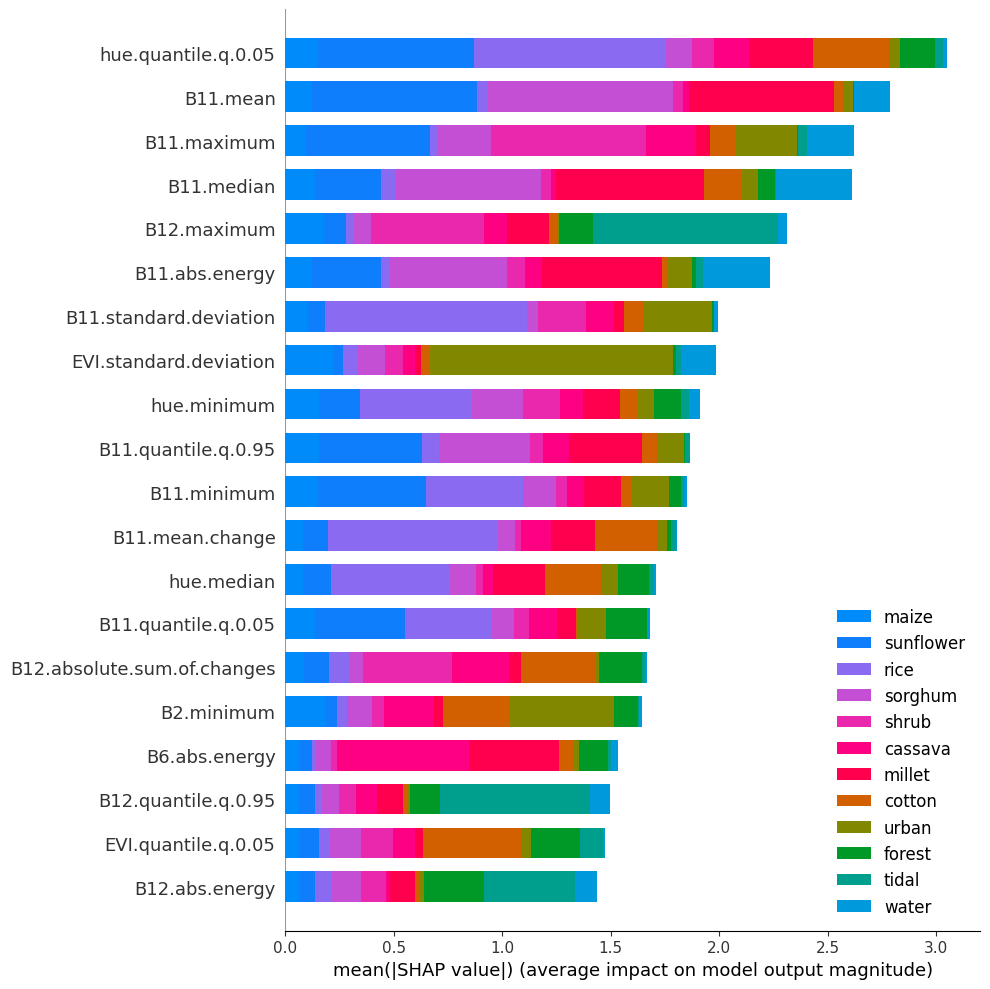
\includegraphics[width=0.8\linewidth]{/home/mmann1123/Documents/github/YM_TZ_crop_classifier/writeup/figures/max_shaps_importance_no_other_30_LGBM_kappa_3.png} % Adjust the path and options
    \caption{Top 20 Max SHAP Feature Importance by Land Cover Type}
    \label{fig:max_shaps} %can refer to in text with \ref{fig:max_shaps}
\end{figure}
 
The final selection of features for model training was carefully curated to include all 30 of both the highest mean and maximum SHAP values, ensuring a comprehensive set of predictors for accurate and reliable classification of crop types in Tanzania. This strategic selection process not only improved model accuracy but also enhanced our understanding of the spectral characteristics most relevant for distinguishing among the diverse agricultural landscapes of the region.

\subsection{Model Selection}
Optuna trials tuning results selected LightGBM \cite{ke2017lightgbm} is a gradient boosting algorithm that combines many simple decision trees to produce a stronger single model, improving the model at each step. LightGBM grows decision trees leaf-wise rather than adding different levels, thereby targeting branches that most need refining.  
\subsection{Model Performance}
The classification model demonstrated robust performance across multiple land cover classes, as evidenced by the out-of-sample mean confusion matrix with a Cohen's Kappa score of 0.82 and F1-micro score of 0.85 (Table \ref{tab:metrics}), indicating substantial agreement between predicted and actual classifications. Remember that each field is treated as a "group" in the group k-fold procedure to ensure that pixels from the same field are not split between the testing and training groups.  The confusion matrix (Figure \ref{fig:oos_confusion}) shows high diagonal values for most classes, highlighting the model's ability to accurately identify specific land covers. For instance, rice and maize achieved out-of-sample classification accuracies of 92\% and 82\%, respectively. Other well-classified categories included millet, sunflower, tidal, water, shrubs, and forest, each with over 73\% accuracy. However forest is primarily confused with the category shrub, which is likely a result of poor training data and the difficulty of visually determining trees versus shrubs from high-res imagery without the benefit of field visits.

Categories such as sorghum, cassava and cotton displayed moderate confusion with other classes, indicating potential areas for model improvement, especially in distinguishing features that are common between similar crop types.  Confusion between cassava and maize might reflect intercropping practices, where cassava is grown alongside other crops, making it difficult to isolate in the satellite imagery. The model's performance on these classes suggests that additional discriminative features or more extensive training data may be necessary to further enhance classification accuracy for these crops.

\begin{figure}[!t] 
    \centering
    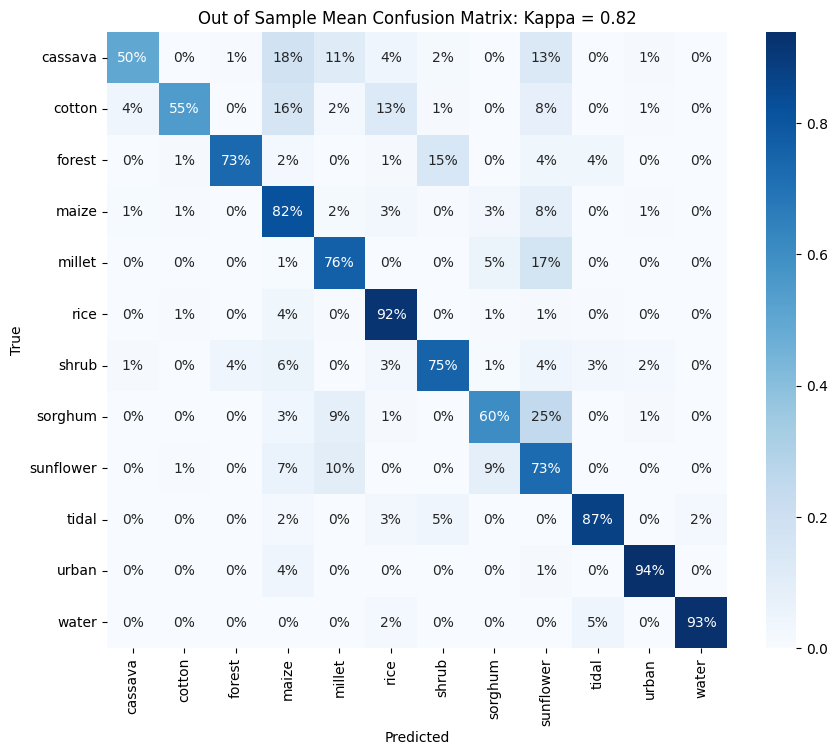
\includegraphics[width=0.8\linewidth]{/home/mmann1123/Documents/github/YM_TZ_crop_classifier/writeup/figures/final_confusion_no_other_model_selection_feature_selection_no_otherLGBM_kappa_3.png} % Adjust the path and options
    \caption{Out of Sample Confusion Matrix}
    \label{fig:oos_confusion} %can refer to in text with \ref{fig:oos_confusion}
\end{figure}

\begin{table} 
\centering
\begin{tabular}{@{}ll@{}}
\toprule
Metric              & Value                 \\ \midrule
Balanced Accuracy   & 0.84    \\
Kappa Accuracy      & 0.82    \\
Accuracy            & 0.85    \\
F1 Micro Accuracy   & 0.85    \\ 
Precision (UA)   & 0.86    \\ 
Recall (PA)   & 0.84    \\ 
\bottomrule
\end{tabular}
\caption{Summary of Classification Metrics}
\label{tab:metrics}
\end{table}

The overall high out-of-sample performance in Table \ref{tab:metrics} across the majority of categories suggests that the model is effective for practical applications in land cover classification, though further refinement is recommended for categories showing lower accuracy and higher misclassification rates.

We can compare our results across multiple models using the figure below in \ref{fig:model_compare} from \cite{kerner2024accurate}. This plot represents multiple performance metrics of land cover models that include an "agricultural" category specifically for Tanzania. Our model’s performance is indicated by the dashed line. The high level of performance - particularly for the more challenging F1 score - is not surprising given that our model is specifically trained on Tanzanian data, while the other models are typically global or regional models. On the other hand, most of these models include only a single ‘agricultural’ class, meaning their prediction task is a significantly easier one than the one presented here. Given this our strong out-of-sample performance is notable.

\begin{figure}[!t]
  \centering
  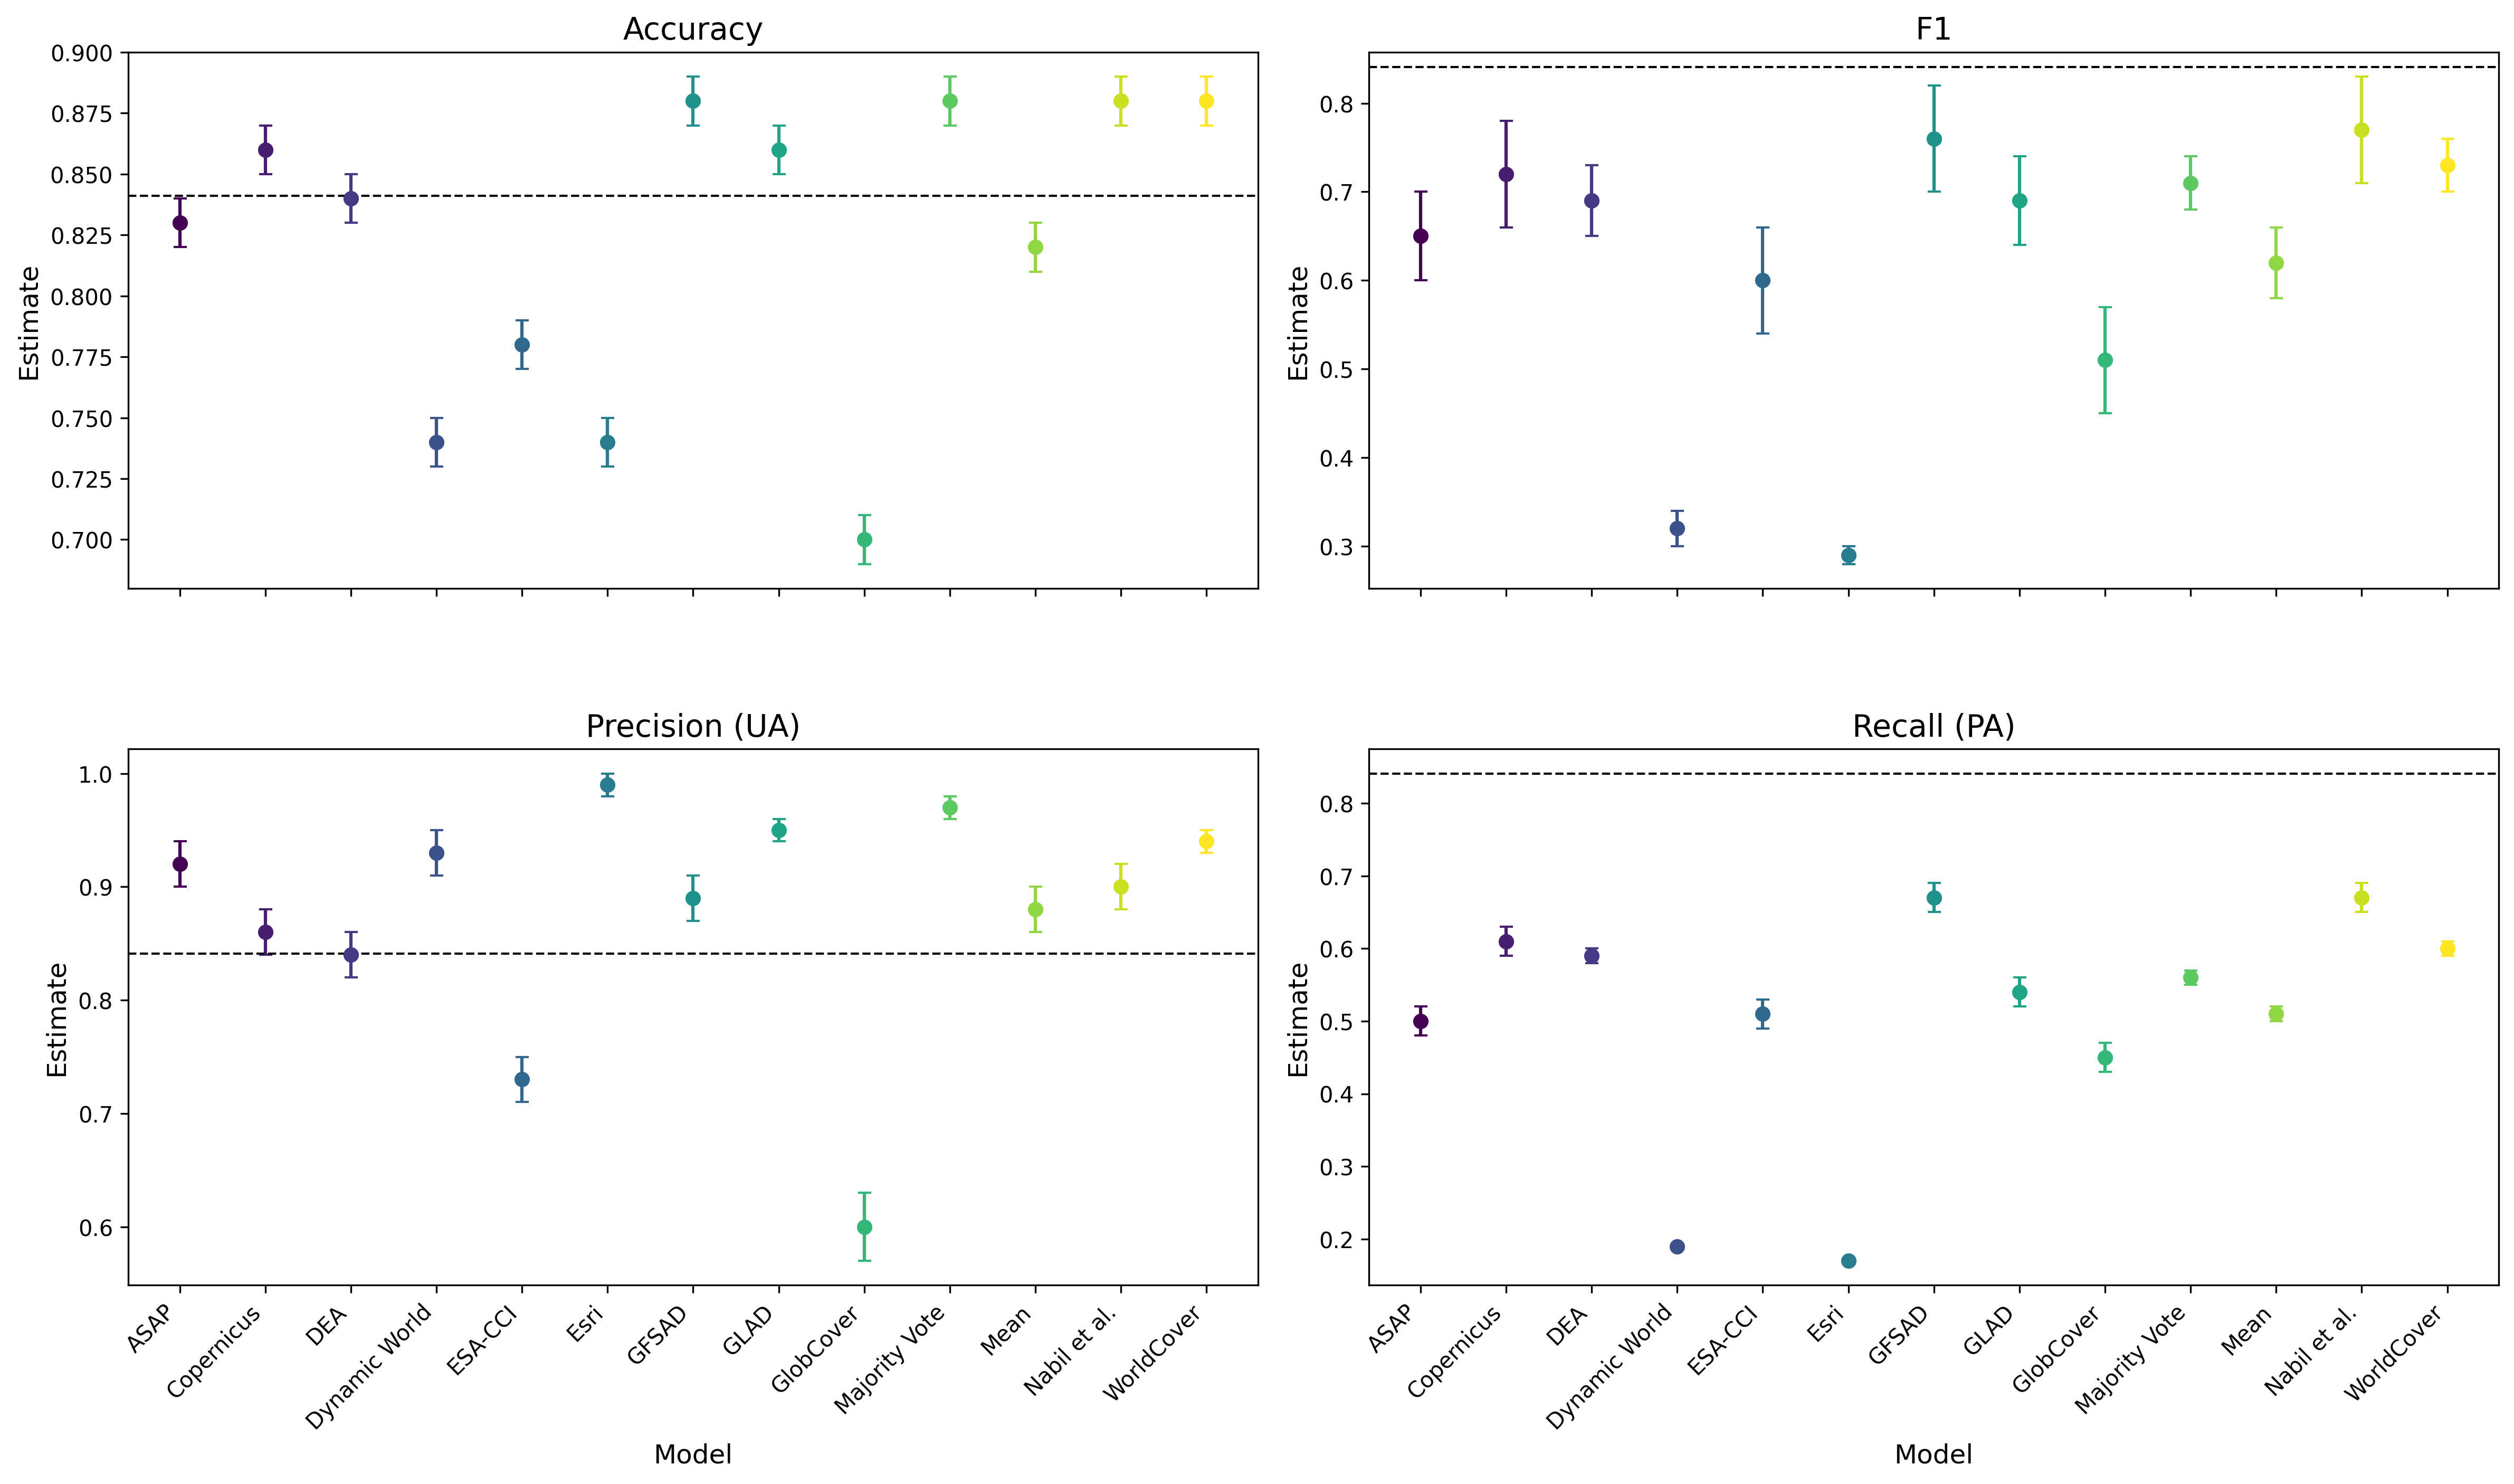
\includegraphics[width=0.8\linewidth]{/home/mmann1123/Documents/github/YM_TZ_crop_classifier/writeup/figures/model_performance.png}  
    \caption{Tanzanian Land Cover Model Performance Comparison - source \cite{kerner2024accurate} \newline Land cover model performance metrics for Tanzania - dashed line indicates this paper’s model out-of-sample performance across all land covers }
    \label{fig:model_compare} %can refer to in text with \ref{fig:model_compare}
\end{figure} 

The integration of crowdsourced data with traditional machine learning and engineered time-series features yielded a robust model for crop classification in Tanzania. While the model performed exceptionally well for crops like maize and rice, some confusion persisted among similar crop types such as sorghum and cotton. This suggests that additional discriminative features or more extensive training data may be necessary to further enhance classification accuracy for these crops. The challenges encountered, such as variability in crop cycles and challenges of crop identification, highlight the complexities of agricultural monitoring in resource-limited settings. Addressing these issues in future research could improve model performance and generalizability. Overall, our findings demonstrate the practicality of using efficient, interpretable machine learning methods in conjunction with community-driven data collection to advance agricultural monitoring in developing regions.

\section{Conclusion}
In this study, we introduced a novel methodology for crop type classification in Tanzania by leveraging crowdsourced data and time-series features extracted from Sentinel-2 satellite imagery. By combining advanced remote sensing techniques with local knowledge, we addressed significant gaps in agricultural monitoring within resource- and data-limited settings. Our approach gathered a new dataset and successfully applied it to a real-world task at very low cost, using traditional machine learning algorithms augmented with carefully engineered time-series features to precisely identify crop types.

Our results demonstrated the effectiveness of the proposed methodology, achieving a Cohen's Kappa score of 0.82 and an F1-micro score of 0.84 across a diverse and multi-class dataset. The model accurately classified challenging crops such as cassava, millet, sorghum, and cotton. The integration of crowdsourced data and time-series features provided valuable insights into the temporal dynamics of crop growth, enhancing the model's accuracy and reliability. Notably, our model—although trained specifically on Tanzanian data—outperforms broadly used land cover models that perform the simpler task of classifying 'agriculture' without specifying the crop type. This highlights the need for better and more frequent crop type classification data.

By interpreting feature importance using SHAP values, we gained a deeper understanding of the model's behavior and the key predictors driving its predictions. Identifying the most influential features across different land cover types allowed us to refine the feature selection process, ensuring that the selected features were both consistently influential and impactful under specific conditions.

In conclusion, our study underscores the viability and effectiveness of traditional machine learning approaches augmented with carefully engineered time-series features for crop type classification in data-scarce environments. By "turning back the clock" on deep learning, we demonstrate that applying a limited yet salient set of filters—such as measures of trends, distribution descriptions, and complexity metrics—can capture essential temporal dynamics without the extensive data requirements of deep learning models. This methodology not only achieved high classification accuracy but also enhanced interpretability and computational efficiency.

Our findings highlight that traditional machine learning techniques, combined with advanced yet computationally efficient feature extraction methods, offer a practical and effective alternative to deep learning, particularly in low-information settings prevalent in developing regions. This approach facilitates accurate crop type classification and contributes valuable insights for sustainable agricultural practices and informed policy-making, ultimately impacting food security and land management in resource-limited contexts.

 

\bibliographystyle{IEEEtran}
\bibliography{/home/mmann1123/Documents/github/YM_TZ_crop_classifier/writeup/refs.bib}




\newpage
% \appendix
\clearpage
\begingroup
\renewcommand{\thepage}{A\arabic{page}}  % Change page numbering for appendix
\setcounter{page}{1}  % Reset page count
\renewcommand{\thesection}{A\arabic{section}} % Change section numbering

\section*{Appendix}

\section{Acknowledgments}
The United States Agency for International Development generously supports this program through a grant from the USAID GeoCenter under Award \# AID-OAA-G-15-00007 and Cooperative Agreement Number: 7200AA18CA00015.

\section{Time Series Features Description}
The following table provides a comprehensive list of the time series features extracted from the satellite imagery using the \texttt{xr\_fresh} module. These features capture the temporal dynamics of crop growth and development, providing valuable information on the phenological patterns of different crops. The computed metrics encompass a wide range of statistical measures, changes over time, and distribution-based metrics, offering a detailed analysis of the temporal patterns in the study area.

\onecolumn
\renewcommand{\arraystretch}{1.5}  
 
\begin{longtable}{|p{4cm}|p{5cm}|p{6cm}|}
\hline
\textbf{Statistic} & \textbf{Description} & \textbf{Equation} \\
\hline
\endhead
Absolute energy &  sum over the squared values & $E = \sum_{i=1}^n x_i^2$ \\
Absolute Sum of Changes  & sum over the absolute value of consecutive changes in the series  & $ \sum_{i=1}^{n-1} \mid x_{i+1}- x_i \mid $ \\
Autocorrelation (1 \& 2 month lag) & Correlation between the time series and its lagged values & $\frac{1}{(n-l)\sigma^{2}} \sum_{t=1}^{n-l}(X_{t}-\mu )(X_{t+l}-\mu)$\\
Count Above Mean & Number of values above the mean & $N_{\text{above}} = \sum_{i=1}^n (x_i > \bar{x})$ \\
Count Below Mean & Number of values below the mean & $N_{\text{below}} = \sum_{i=1}^n (x_i < \bar{x})$ \\Day of Year of Maximum Value & Day of the year when the maximum value occurs in series & --- \\
Day of Year of Minimum Value & Day of the year when the minimum value occurs in series & --- \\
Kurtosis & Measure of the tailedness of the time series distribution & $G_2 = \frac{\mu_4}{\sigma^4} - 3$ \\
Linear Time Trend & Linear trend coefficient estimated over the entire time series & $b = \frac{\sum_{i=1}^n (x_i - \bar{x})(t_i - \bar{t})}{\sum_{i=1}^n (x_i - \bar{x})^2}$ \\
Longest Strike Above Mean & Longest consecutive sequence of values above the mean & --- \\
Longest Strike Below Mean & Longest consecutive sequence of values below the mean & --- \\
Maximum & Maximum value of the time series & $x_{\text{max}}$ \\
Mean & Mean value of the time series & $\bar{x} = \frac{1}{n}\sum_{i=1}^n x_i$ \\
Mean Absolute Change & Mean of absolute differences between consecutive values & $\frac{1}{n-1} \sum_{i=1}^{n-1} | x_{i+1} - x_{i}|$ \\
Mean Change & Mean of the differences between consecutive values & $ \frac{1}{n-1} \sum_{i=1}^{n-1}  x_{i+1} - x_{i} $ \\
Mean Second Derivative Central & measure of acceleration of changes in a time series data & $\frac{1}{2(n-2)} \sum_{i=1}^{n-1}  \frac{1}{2} (x_{i+2} - 2 \cdot x_{i+1} + x_i)
$ \\
Median & Median value of the time series & $\tilde{x}$ \\
Minimum & Minimum value of the time series & $x_{\text{min}}$ \\
Quantile (q = 0.05, 0.95) & Values representing the specified quantiles (5th and 95th percentiles) & $Q_{0.05}, Q_{0.95}$ \\
Ratio Beyond r Sigma (r=1,2,3) & Proportion of values beyond r standard deviations from the mean & $P_r = \frac{1}{n}\sum_{i=1}^{n} (|x_i - \bar{x}| > r\sigma_{x})$ \\
Skewness & Measure of the asymmetry of the time series distribution & $\frac{n}{(n-1)(n-2)} \sum \left(\frac{X_i - \overline{X}}{s}\right)^3$ \\
Standard Deviation & Standard deviation of the time series & $  \sqrt{\frac{1}{N}\sum_{i=1}^{n} (x_i - \bar{x})^2}$ \\
Sum Values & Sum of all values in the time series & $S = \sum_{i=1}^{n} x_i$ \\
Symmetry Looking & Measures the similarity of the time series when flipped horizontally & $| x_{\text{mean}}-x_{\text{median}} | < r * (x_{\text{max}} - x_{\text{min}} ) $ \\
Time Series Complexity (CID CE) & measure of number of peaks and valleys & $\sqrt{ \sum_{i=1}^{n-1} ( x_{i} - x_{i-1})^2 }$\\
Variance & Variance of the time series & $\sigma^2 = \frac{1}{N}\sum_{i=1}^{n} (x_i - \bar{x})^2$ \\
Variance Larger than Standard Deviation & check if variance is larger than standard deviation & $\sigma^2 > 1$ \\
\hline
\end{longtable}


\twocolumn
\endgroup


\end{document}





